\documentclass[11pt]{article}
\usepackage[T1]{fontenc}	%special characters
\usepackage[utf8]{inputenc}	%special characters
\usepackage{lmodern,textcomp}% Euro Symbol

\usepackage{hyperref}
\usepackage[margin=1in]{geometry} %article layout margins
\usepackage{tabularx}		%tabulars width fixed textwidth
\usepackage{multicol}	%2 columns in Skills
\usepackage{graphicx}
\usepackage{sectsty}
\sectionfont{
	\sectionrule{0pt}{0pt}{-5pt}{0.8pt}
}

\begin{document}

\Large
\noindent
\textbf{Dirk Hornung, Ph.D.} \\

\normalsize
\noindent
\begin{minipage}{0.5\linewidth}
  \begin{tabularx}{0.6\textwidth}{>{\bfseries}l l}
    City:           & Barcelona \\
    Date of birth:  & October 5, 1991\\
    Place of birth: & Fulda, Germany \\
    Mobile:         & +34 695460404 \\
    E-mail:         & hello@drdirk.io \\
    Website:      	& drdirk.io
  \end{tabularx}
\end{minipage}
\begin{minipage}{0.5\linewidth}
  \begin{flushright}
    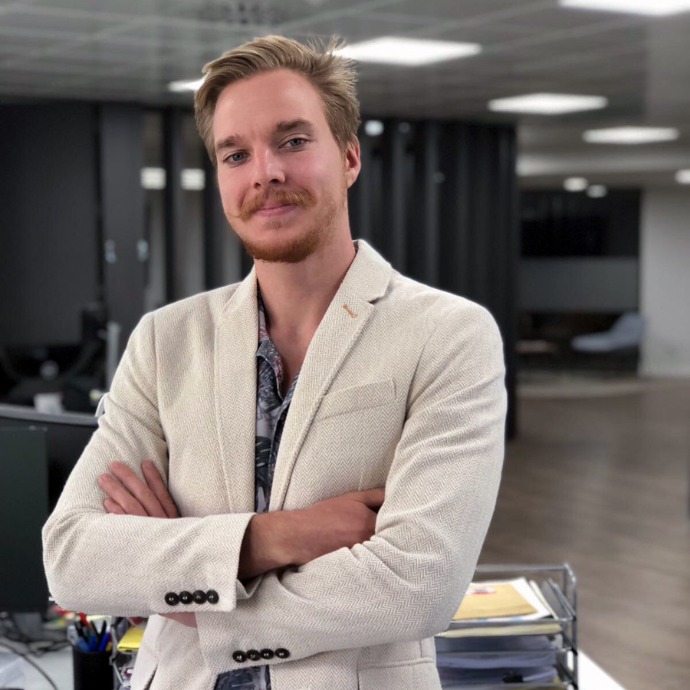
\includegraphics[width=0.4\textwidth]{dirk.png}
  \end{flushright}
\end{minipage}

 \section*{}
 \vspace{1cm}


 % FRENCH
 % Je suis Dirk Hornung récemment diplômé en physique theorique. J'ai
 % étudié à l'institut de physique des hautes énergies de l'Université autonome de
 % Barcelone et l'Université d'Aix-Marseille. J'ai plus de 5 ans d'expérience dans
 % la gestion de la technologie dans différentes startups mais cherche de
 % developer ma carrière comme Data Scientist. Dans mes études, j'ai déja pris de
 % experience avec le analyse de données: J'ai développé une
 % routine en C++ pour extraire les paramètres de
 % modèles théoriques à partir de données expérimentales. J'ai utilisé des outils
 % de données tels que pandas, matplotlib et scipy. \\

 % \noindent En plus de mes études, je suis un entrepreneur. Au cours de la
 % dernière année, j'ai développé des contrats intelligents dans la Blockchain
 % Ethereum avec une API REST utilisant Node Express pour un legaltech. Avant j'ai
 % développé un chatbot en utilisant l'Intelligence artificielle pour une fintech,
 % où j'étais responsable du naturel Traitement de la langue. un développeur
 % Full-stack avec beaucoup de expérience en développement d'applications en
 % utilisant React comme interface et noeud dans

 % \noindent Je suis actuellement en train de m'éduquer sur le thème de
 % l'artificiel Intelligence et apprentissage automatique, en particulier dans le
 % domaine de la formation en profondeur Apprentissage. J'ai récemment terminé
 % Coursera Deep Learning d'Andrew Ng Spécialisation. En dehors de cela, je
 % pratique mon Tensorflow et Compétences en keras dans l'onde sonore de python
 % simulations et annulation active du bruit.
 %%%%%%%%%%%%%%%%%%%%%%%%%%%%%%%%%%%%%%%%%%%%%%%%%%%%%%%%%%%%%%%%%%%%%%%%%%%%%%%


 % English
 Dear TNG Technology Consulting, \\

 \noindent I am Dirk Hornung, a recently graduated Ph.D. student at
 the institute of high energy physics of the Autonomous University of
 Barcelona with 5+ years of experience in leading the technology in
 different Startups. Within my studies, I researched low-energy QCD
 and the determination of Standard Model parameters. I developed a C++
 fitting routine to extract parameters of
 theoretical models out of CERN experimental data. \\

 \noindent Besides my studies, I am an entrepreneur. During the last year, I
 developed Smart Contracts in the Ethereum Blockchain and connected them through
 REST APIs using Node Express for a legaltech. Before I developed a chatbot
 using Artificial Intelligence for a fintech. We connected our clients through
 Messenger to their bank accounts and analyzed their banking information using
 Python. I am furthermore a Full-stack developer with lots of experience
 developing applications using React as frontend and AWS services as a backend.  \\

 \noindent Currently I am educating myself on the topic of Artificial Intelligence
 and Machine Learning, especially in the field of Deep Learning. I recently completed
 Andrew Ng's Coursera Deep Learning Specialization. Apart from that, I am practising my
 Tensorflow and Keras skills within python sound wave simulations and active noise cancelling.\\

 \noindent Sincerely, \\
 Dr. Dirk Hornung \\

 \noindent P.S. I am a native German, but also fluent in English, French and
 Spanish. Visit drdirk.io to get to know me better.

 \end{document}